\chapter{Techniques for reducing output mode cleaner beam jitter noise}
\label{ch:jitter}
When using an OMC in the readout of an interferometer, probably the most important new source of noise to arise is beam jitter. %NL%
A related form of beam jitter noise also exists in the arm cavities of an interferometer \cite{Kawamura:94}. %NL%
Fluctuations of the output beam are however not generally an issue with an interferometer that does not use an OMC, so long as the beam apertures are always sufficient to prevent beam clipping. %NL%


An OMC may perform very well as a spatial filter for unwanted higher order modes, but simultaneously it becomes very sensitive to pointing fluctuations of the input beam. %NL%
The GEO600 OMC which was tested by LIGO was placed outside of vacuum, and beam jitter noise ruined the sensitivity in most of the measurement band. %NL%
It was for this reason that the Enhanced LIGO OMC was placed in vacuum \cite{G040326}. %NL%
Even with this improvement, much time and effort was spent by the commissioning teams in Enhanced LIGO to locate and remove sources of beam jitter noise. %NL%
This Chapter will cover much of what was learned regarding beam jitter noise during the commissioning of Enhanced LIGO.

\section{The noise mechanism of beam jitter incident on a high finesse cavity}

Motion of the beam incident on a high finesse cavity alters the overlap of said beam with the resonant mode of the cavity. %NL%
This leads to fluctuations in the amount of light which can couple into the cavity and consequently, power fluctuations of the transmitted beam. %NL%
The power fluctuation can spoil the measurement of the intrinsic amplitude modulation of the beam if the measurement and fluctuations occur at the same frequencies.

For a beam incident on the cavity which has a lateral (perpendicular to the direction of propagation) and angular misalignment, constrained to a plane, we have the following expression for the power transmitted through the cavity
\begin{equation}
\label{eqn:simplejitter}
P\approx P_0\left(1-\left(\frac{\Delta x}{w_0}\right)^2-\left(\frac{\theta}{\theta_d}\right)^2\right),
\end{equation}\com{This is correct, check for consistency, also with modal model chap}
where $P_0$ is the power transmitted of the aligned beam, $\Delta x$ is the beam waist displacement, $\theta$ is the beam waist tilt, $w_0$ is the beam waist radius, and $\theta_d$ is the divergence angle of the beam. %NL%
The approximation holds while both the angular and lateral misalignments are small.

Equation \ref{eqn:simplejitter} shows that beam misalignments couple to the transmitted power quadratically. %NL%
This leads to a few relevant consequences. %NL%
The coupling of beam jitter to transmitted power is nonlinear, thus frequency components of the beam motion may be mixed together, producing new frequencies in the transmitted power. %NL%
Also, the linear coupling coefficient of beam jitter to power fluctuations is proportional to the DC beam misalignment. %NL%
This causes the direct linear coupling of frequency components of beam jitter to power fluctuations to vary as the DC pointing error varies.

Steering optics in the beam path leading to the cavity which are vibrating may transfer vibrations to the laser beam and produce beam jitter noise. %NL%
Let us investigate beam jitter coupling of an optic in the modal picture. %NL%
 We will work in a basis of only the \TEM{00} and \TEM{01} modes. %NL%
Let's assume we have a beam which is dominantly in the \TEM{00} mode as measured in the basis of our cavity, with some small amplitude of \TEM{01} mode. %NL%
In other words, we begin with a beam which is slightly misaligned.
\begin{equation}
\vect{E}_{\text{input}}=E_0\left(\vect{00}+\alpha\vect{01}\right).
\end{equation}
The misalignment, $\alpha$ may be do to another steering mirror upstream, or a misalignment of the beam source relative to our cavity axis, the precise origin is not critical for this discussion.

Now we will assume this beam is incident on a steering mirror before it finally enters the cavity. %NL%
This steering mirror also has a slight misalignment, $\theta$. %NL%
Equation \ref{eqn:mirrortilt} shows the matrix representing the operator of a mirror which has been tilted from nominal alignment. %NL%
The beam incident on the cavity is then
\begin{equation}
\vect{E}_{\text{incident}}=\oper{M}(\Theta)\vect{E}_{\text{input}},
\end{equation}
where, as before, $\Theta=\frac{\theta \pi w(z)}{\lambda}$, while $w(z)$ is the beam width radius at the mirror, and $\lambda$ is the laser wavelength. %NL%
Because the cavity has a high finesse, when the cavity is resonant on the \TEM{00} mode, only that mode is transmitted. %NL%
Thus, for the field transmitted by the cavity
\begin{equation}
E_{\text{t}}=t_{\text{cavity}}\matrixel{00}{\oper{M}\left(\Theta\right)}{E}_{\text{input}}=t_{\text{cavity}}E_0\left(1-i\frac{ \pi w(z)}{\lambda}\theta\alpha\right),
\end{equation}
where $t_{\text{cavity}}$ is the amplitude transmission of the cavity. %NL%
This causes a power fluctuation on transmission
\begin{equation}
\label{eqn:mirrorjitter}
P=E_t^*E_t=P_0\left(1+\frac{2\pi w(z)}{\lambda}\theta\Im(\alpha)\right),
\end{equation}
where $P_0=|t_{\text{cavity}}E_0|^2$. %NL%
Only the imaginary part of $\alpha$ contributes to beam jitter noise of our mirror because it represents an error in alignment \emph{angle}, not position, at the location of the steering mirror $\oper{M}$. %NL%


One interesting consequence of Equation \ref{eqn:mirrorjitter} is that for a given mirror, the strength of beam jitter coupling is proportional to $w(z)$, the size of the beam on the optic. %NL%
Thus one technique for reducing beam jitter coupling is to design one's optical path in such a way that beams are smaller on optics that may produce significant beam jitter. %NL%
This of course also reduces their efficiency as an alignment control mirror.

Furthermore, we again see a nonlinear coupling in the form of mixing of the incident misalignment, $\alpha$, and the jitter of the steering mirror, $\theta$. %NL%
We may suppose that the input alignment has both a DC component and possibly some low frequency (a few to several Hz) wandering motion. %NL%
If this is coupled with high frequency (i.e. %NL%
frequencies in the detection band) jitter of the steering mirror, the mixing of frequencies can cause noise in the power transmission at and around the jitter frequency of the steering optic.

\begin{figure}
  \begin{center}
  \leavevmode
  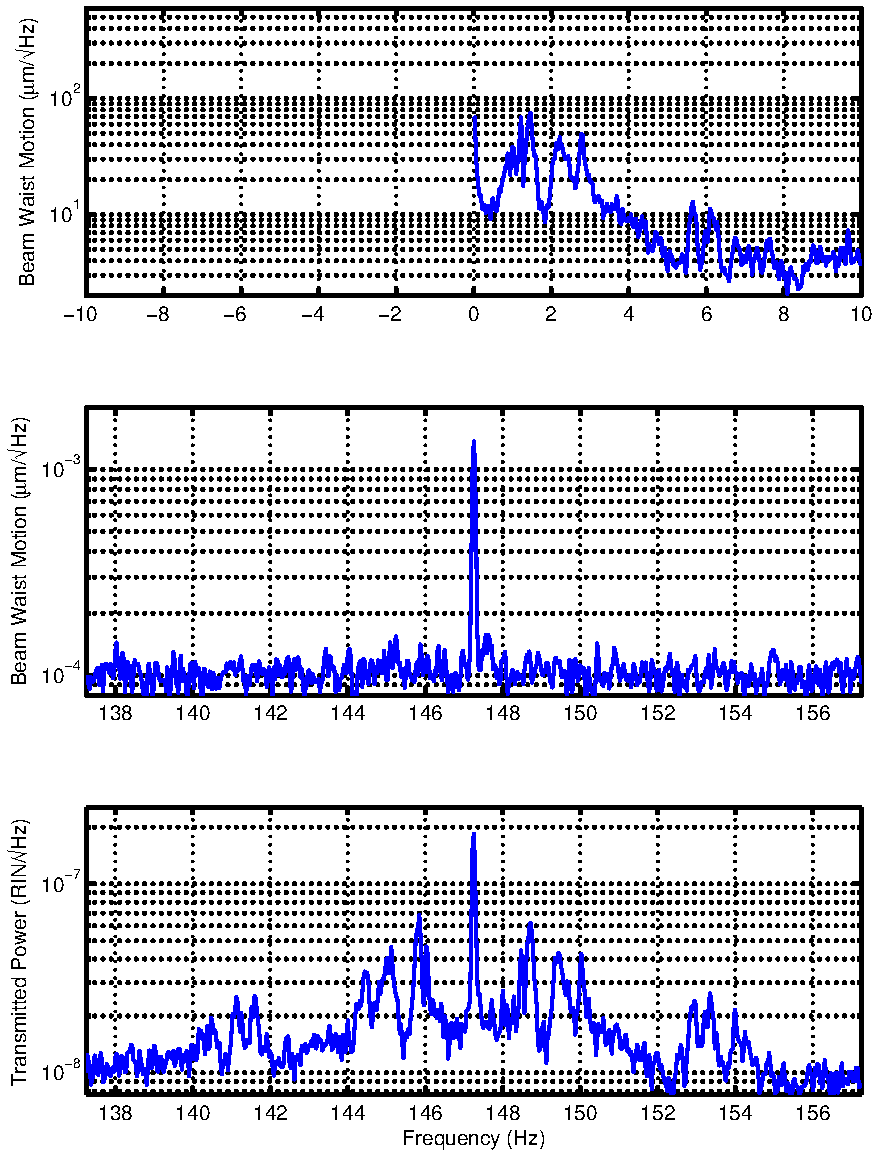
\includegraphics{figs-jitter/bilinearplot.pdf}
  \end{center}
  \caption[Measurement of the bilinear coupling of beam jitter noise.]{Measurement of the bilinear coupling of beam jitter noise. The top panel shows low frequency beam motion measured by the OMC input QPDs. Shown in the center panel is an audio frequency beam jitter peak, this peak was shown to arise from a vacuum scroll pump outside of the HAM6 chamber \cite{robert147}. The bottom panel shows how the low frequency motion has been imparted as sidebands on a central beam jitter peak in the OMC transmitted light.}
  \label{fig:bilinear}
\end{figure}

With the introduction of the OMC in Enhanced LIGO, bilinear beam jitter coupling became a much more prominent source of noise. %NL%
Figure \ref{fig:bilinear} shows how low frequency beam motion mixes with high frequency jitter to produce broad sidebands around beam jitter peaks. %NL%
This is similar to how beam jitter was discussed by \citet{Tobin}.

\section{Mechanical resonances of beam steering optics}
When the Enhanced LIGO interferometers were first performing at a sensitivity comparable to the state of the interferometers in the S5 science run, there were large glaring peaks in the sensitivity spectrum. %NL%
It was determined fairly quickly that these were due beam jitter, but the mechanism causing the jitter was unknown.

The Enhanced LIGO upgrade introduced several modifications to the readout chain of the interferometer. %NL%
As discussed in Chapter \ref{ch:omc}, with the introduction of the in-vacuum OMC, it was necessary to use new beam steering and mode matching optics to couple the beam exiting the interferometer to the OMC cavity. %NL%
These steering optics, as well as the OMC, were all housed in a single vacuum chamber on top of the prototype HAM ISI platform which is planned to be used copiously in Advanced LIGO. %NL%
Although it was not fully appreciated at the start of Enhanced LIGO, the new isolation platform provided much reduced vibration isolation at audio frequencies when compared to the isolation tables used in the HAM chambers in Initial LIGO. %NL%
Figure \ref{fig:hamtransmission} shows a comparison of the transmission of ground motion to motion of the HAM table for both the initial LIGO passive isolation system, and the Enhanced LIGO HAM ISI.

\begin{figure}
  \begin{center}
  \leavevmode
  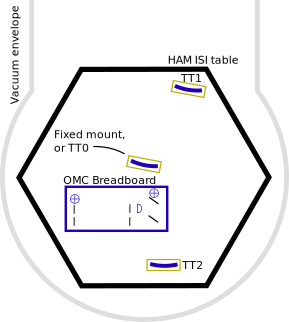
\includegraphics{figs-jitter/ham6layout.pdf}
  \end{center}
  \caption[Schematic of HAM6 optical layout.]{Schematic of HAM6 optical layout. The beam which exits the interferometer antisymmetric port is directed by three steering mirrors onto the OMC. The first steering mirror was originally a fixed post, and changed later to a passive suspended Tip Tilt optic. The second and third Tip Tilts were known used for active beam steering control. A small fraction of the light incident on the OMC transmits through a highly reflective steering mirror and is sensed by two quadrant photodetectors.}
  \label{fig:ham6layout}
\end{figure}

\begin{figure}
  \begin{center}
  \leavevmode
  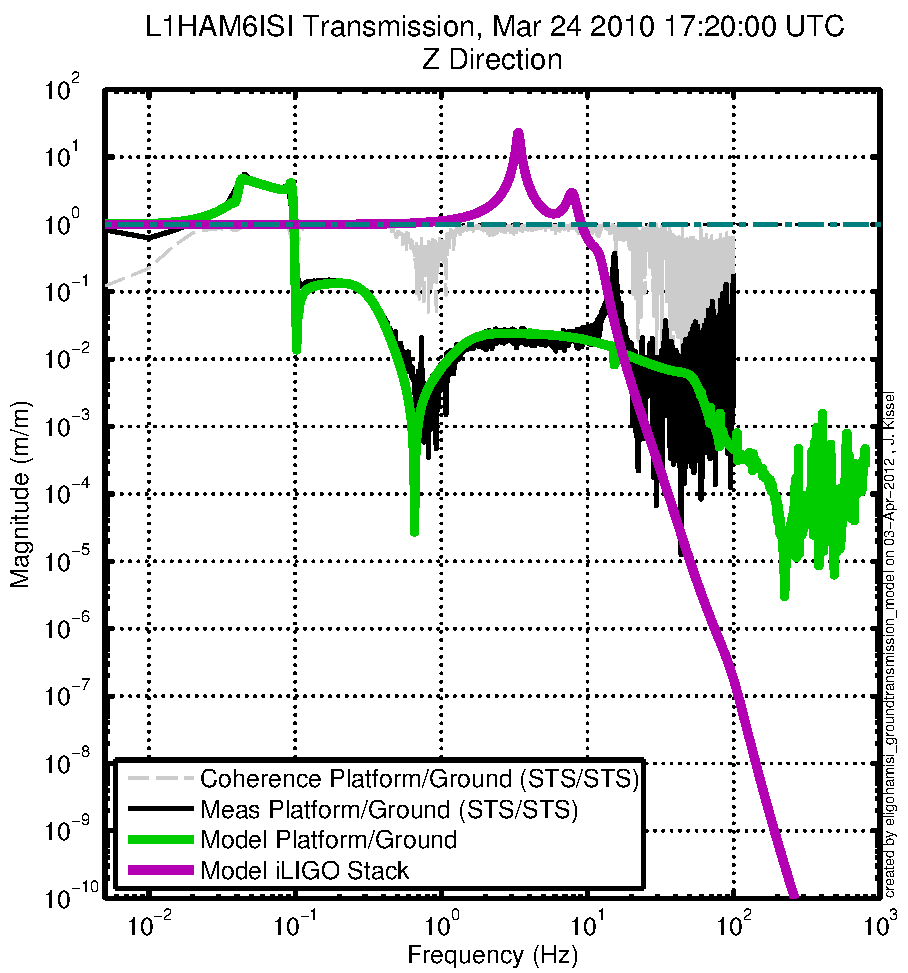
\includegraphics{figs-jitter/hamtransmission.pdf}
  \end{center}
  \caption[Comparison of vertical vibrational motion transmission of the Initial and Enhanced LIGO HAM chamber isolation systems.]{Comparison of vertical vibrational motion transmission of the Initial and Enhanced LIGO HAM chamber isolation systems. While the low frequency isolation of the HAM ISI is far superior to that of the old passive stack, in the most sensitive region of the interferometer (100-200Hz), the HAM ISI transmits a few orders of magnitude greater than the passive system. The high frequency behavior of the HAM ISI model (green curve) represents true resonant structure and is not a result of measurement noise. Credit and appreciation for this figure goes to Jeff Kissel.}
  \label{fig:hamtransmission}
\end{figure}

The optical layout of the OMC chamber of Enhanced LIGO comprised three steering optics, which also behaved as a mode matching telescope, and the OMC itself. %NL%
In the initial configuration, the first of these was a mirror on a fixed mount, while the other two were in a Tip-Tilt suspension system with active beam steering. %NL%
A diagram of the optical layout is shown in Figure \ref{fig:ham6layout}. %NL%
Diligent work by Robert Schofield determined that some of the largest beam jitter peaks degrading the interferometer sensitivity were due to vibrations of the fixed mirror mount \cite{fixedmountpeaks}. %NL%
To rectify this situations, the fixed mirror mount was replaced with a small mirror suspension similar to the Tip Tilts but without the active steering control. %NL%
Comparison of the old and new designs are shown in Figure \ref{fig:TT0photos}. %NL%
This new style was referred to as the passive Tip Tilt, or TT0. %NL%
As seen in Figure \ref{fig:sensimprovement}, this was effective at removing the largest peaks, though some new peaks appeared in the 150-200Hz region.

\begin{figure}
  \begin{center}
  \leavevmode
  \includegraphics{figs-jitter/TT0photos.pdf}
  \end{center}
  \caption[The evolution of the passive Tip Tilt.]{The evolution of the passive Tip Tilt. These photos show several stages in the configuration of the first mode matching/steering mirror used in HAM6. The original design was an optic mount attached to a fixed post, shown in the left panel. This was later changed (shown in center panel) to a passively suspended version, made by University of Florida, designed by M. Meyer at LIGO Livingston based on the original active Tip Tilt design. The right panel shows a further re-design where the upper suspension wire clamps are attached by blade springs to the suspension cage.}
  \label{fig:TT0photos}
\end{figure}

The origin of the peaks located in the most sensitive region of the LIGO sensitivity spectrum (``the bucket'') was finally determined by a measurement of the coupling of motion from the table to the pointing of the laser beam itself. %NL%
The OMC was equipped with a pair of quadrant photodetectors (QPDs) which sampled the beam incident on the OMC. %NL%
These QPDs were used to measure the response of the beam motion to motion of the ISI table, which is measured by inertial sensors built into the table. %NL%
A measurement of the transfer function of table motion to beam motion may be seen in Figure \ref{fig:TTbounceTF}. %NL%
The resonances were determined to be the bounce (vertical) and roll (rotation about the beam axis) modes of the Tip Tilt optics \cite{tt1bounce}.

\begin{figure}
  \begin{center}
  \leavevmode
  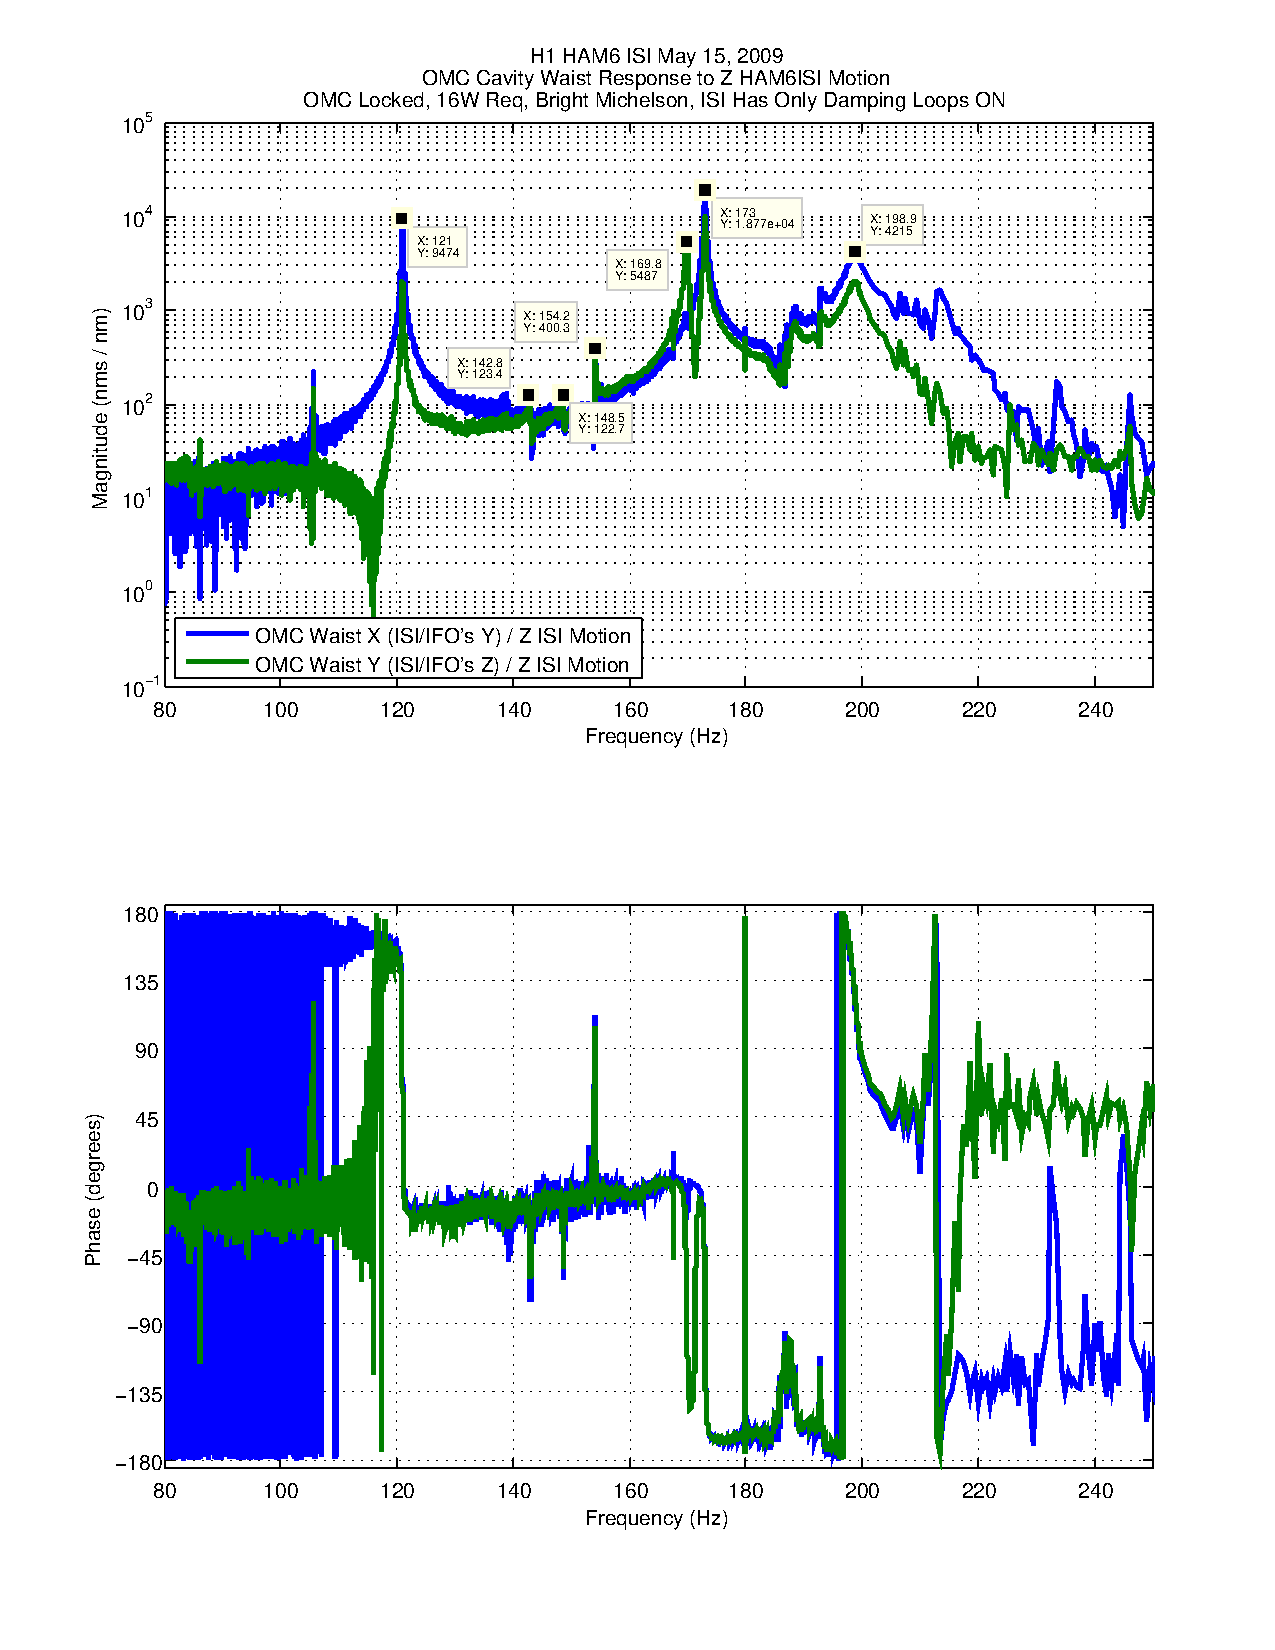
\includegraphics[width=\textwidth]{figs-jitter/TTbounceTF.pdf}
  \end{center}
  \caption[Measurement of HAM table motion coupling to beam motion.]{Measurement of HAM table motion coupling to beam motion. This measurement was performed while all three Tip Tilts used thick suspension wires and no blade springs. This measurement provided evidence that it was the optics on HAM6 which were causing beam jitter peaks in the sensitivity curve of the interferometer.}
  \label{fig:TTbounceTF}
\end{figure}

\begin{figure}
  \begin{center}
  \leavevmode
  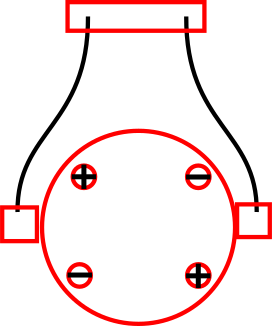
\includegraphics{figs-jitter/ttdiag.pdf}
  \end{center}
  \caption[Diagram of the Tip Tilt suspension with thick wires.]{Diagram of the Tip Tilt Suspension with thick wires. The thickness of the wires caused them to hang with a curve (the curve is exaggerated in this Figure), which lowered the vertical resonance frequency relative to straight wires. Also shown is the relative polarity of the permanent magnets used for active beam steering control.}
  \label{fig:ttdiag}
\end{figure}

The Tip Tilt design had originally assumed the vertical restoring force was due only to stretching tension in the wires. %NL%
The vertical resonance was expected to lie near the 340Hz violin resonances of the main interferometer test mass suspensions, which were already In fact, the wires had a diameter of $380\upmu \rm m$ which was sufficient to cause the break off point of the suspension to be far from the wire clamp. %NL%
Instead of being straight, the wires took more of an `S' shape, as shown in Figure \ref{fig:ttdiag}. %NL%
The bend in the wire resulted in giving the wire much more yield, reducing the resonant frequencies and placing them directly in the most sensitive region of LIGO. %NL%
A finite element analysis of resonances of optics suspended by curved optics was performed by Matt Evans and supported this general theory \cite{mattfea}.

\begin{figure}
  \begin{center}
  \leavevmode
  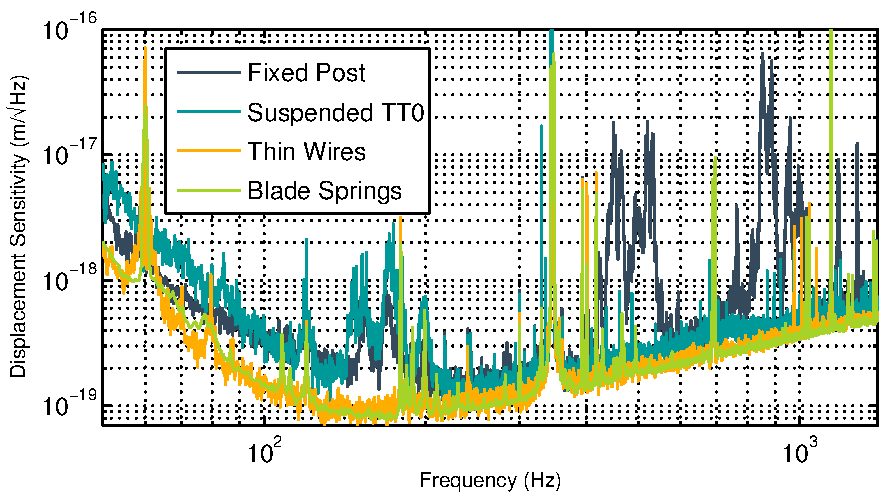
\includegraphics{figs-jitter/sensimprovement.pdf}
  \end{center}
  \caption[Measurement of interferometer sensitivity for different Tip Tilt designs.]{\com{thicken lines} Measurement of interferometer sensitivity for different Tip Tilt designs. Changing the configuration of TT0 from a fixed post to a suspended optic removed large features in the 400-1000Hz region, but increased the noise in the 150-200Hz region. Most features were removed when all Tip Tilts were suspended by thin wires. Finally the configuration was changed again to use blade springs due to the fragility of the thin wires, this also removed the vertical resonance of TT1 near 80Hz. Changes in the background noise floor are not due to modifications of the Tip Tilts.}
  \label{fig:sensimprovement}
\end{figure}

The Tip Tilt suspension was first modified by using thinner wires of radius $50 \upmu \rm m$. %NL%
This had the desired effect of reducing the frequency of the bounce resonance to be below the sensitive measurement band \cite{smallwirecoupling}, but could not function as a permanent solution due to the fragility of the wires.\footnote{One of the Tip Tilts doubled as a fast beam diverter to protect the OMC photodiodes from the full stored energy of the arm cavities which exits the AS port when the interferometer loses lock. %NL%
This system would put considerable force on the suspension and after several lock loss cycles it broke one of the Tip Tilt suspension wires. %NL%
The wire radius was increased to $75 \upmu \rm m$ until the blade spring design was ready for installation.} The ultimate solution was to place the upper wire clamps at the ends of blade springs. %NL%
The new Tip Tilt assembly is shown in Figure \ref{fig:TT0photos}. %NL%
This reduced the vertical resonances to near 20Hz \cite{bladebounce,bladebounceLHO}, outside of the sensitive region, but while still allowing the use of wires with enough strength. %NL%
The sensitivity of the interferometer after this change was made is shown in Figure \ref{fig:sensimprovement}. %NL%
Some amount of high frequency acoustic coupling was re-introduced with the blade springs, likely due to strong passive damping of the vertical eigenmodes with Viton rubber \cite{G1100330}, though it was not a limiting noise source.

Mechanical resonances of optic supports in the beam path should stay in the front of the mind of those investigating sources of beam jitter noise. %NL%
Determining the precise source is certainly helped by having the luxury of an optics table equipped with position sensors and an actuation system.
\section{Magnetic field coupling and feed forward subtraction}
Even after the mitigation of mechanical beam jitter on the OMC, there was still significant pollution of the LIGO sensitivity at frequencies surrounding 60Hz. %NL%
60Hz is the frequency of the AC power distribution system in the U.S.A. %NL%
and is a well known source of trouble to those attempting to do precision measurement. %NL%
It is not terribly troublesome if 60Hz interference into one's device is fairly narrow-band. %NL%
During Enhanced LIGO commissioning however, the 60Hz line was surrounded by broad sidebands which were inferred to be caused by beam jitter. %NL%
This was particularly troubling because of the importance of sensitivity to gravitational wave emission from the Crab pulsar, which is expected to emit gravitational waves at 59.56Hz \cite{Crab}.

The Tip Tilt suspensions utilized permanent magnets affixed to the optics and coil electromagnets for active beam steering control. %NL%
The four permanent magnets were arranged on the face of the optic as shown in Figure \ref{fig:ttdiag}. %NL%
The polarities were alternated so that uniform ambient magnetic fields would not cause a force or torque on the optic. %NL%
Robert Schofield determined that the source of the beam jitter peaks at multiples of 60Hz were in fact due to \emph{gradients} in the ambient magnetic field at those frequencies \cite{60Hzgrad}. %NL%
He also suggested that the use of a magnetometer sensor outside of the vacuum chamber would provide a signal that could be applied to the Tip Tilt alignment control and cancel the effects of the ambient field \cite{60hzff}. %NL%
In addition, the strength of the permanent dipole magnets used in the Tip Tilts was reduced.

\begin{figure}
  \begin{center}
  \leavevmode
  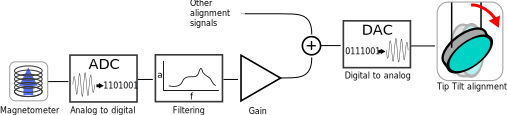
\includegraphics{figs-jitter/magffblockdiag.pdf}
  \end{center}
  \caption[Block diagram of the magnetometer feed forward system.]{Block diagram of the magnetometer feed forward system. The signal read by an analog magnetometer is digitized and filtered. The signal is then combined with other digital alignment signals, converted to analog, and applied to the Tip Tilt alignment actuators.}
  \label{fig:magffblockdiag}
\end{figure}

A magnetometer was installed and a feed forward control system was implemented in the LIGO real time system for digital signal processing. %NL%
The feed forward system read the digitized 3-axis magnetometer signal, performed filtering, and fed the filtered signal to the Tip Tilt pitch and yaw actuators. %NL%
A diagram of the system may be seen in Figure \ref{fig:magffblockdiag}. %NL%


\begin{figure}
  \begin{center}
  \leavevmode
  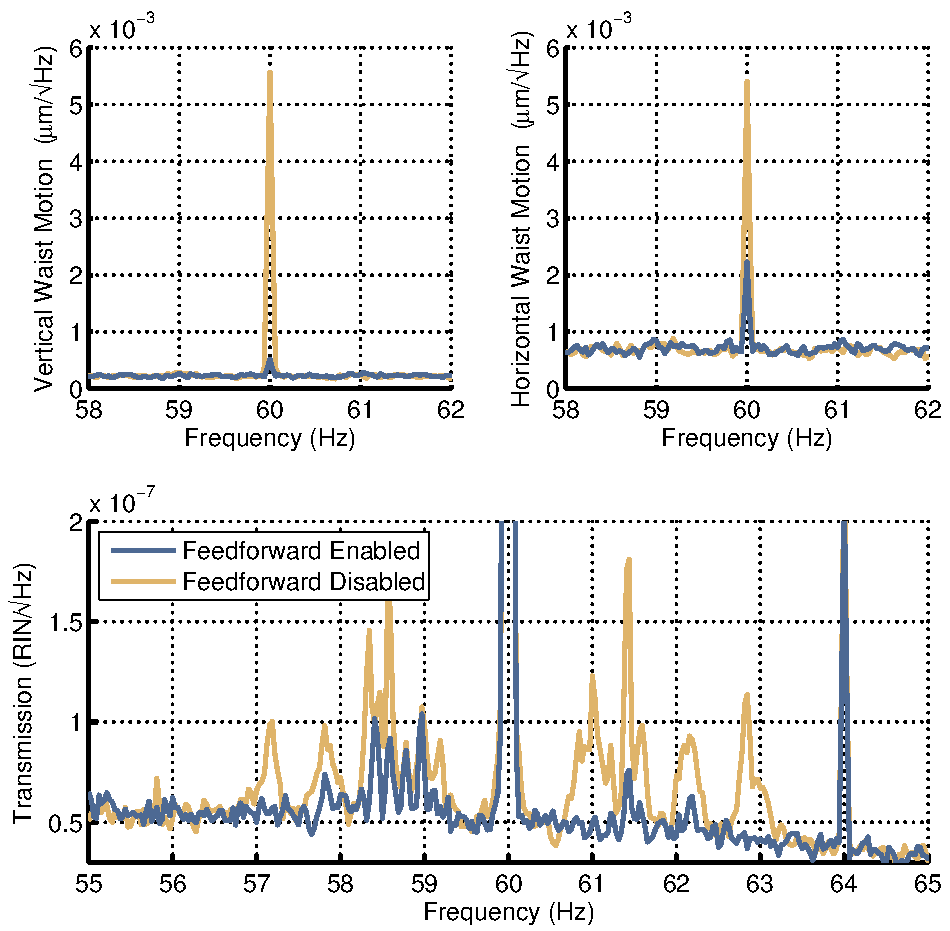
\includegraphics{figs-jitter/magffperformance.pdf}
  \end{center}
  \caption[Measurement of the performance of the magnetometer feed forward system.]{Measurement of the performance of the magnetometer feed forward system. The feed forward system was tuned to minimize the beam motion as measured by the OMC quadrant photodetectors (shown in both top panels). The beam jitter reduction leads to a reduction of the highly variable sidebands structures around the 60Hz line.}
  \label{fig:magffperformance}
\end{figure}

To reduce the 60Hz jitter peak, the signal filtering was tuned to minimize the presence of 60Hz motion measured by the OMC QPDs. %NL%
When correctly tuned, the feed forward system was able to significantly reduce the magnitude of the sidebands around 60Hz in the LIGO sensitivity spectrum. %NL%
The performance of the magnetometer feed forward system is shown in Figure \ref{fig:magffperformance}.

Such a feed forward servo is beneficial whenever one has a signal which is coherent with the source of high frequency jitter noise. %NL%
Because of the bilinear coupling of beam jitter, removal of even narrow, single frequency, components of beam motion can reduce broadband sources of noise in one's data. %NL%
With only the magnetometer signal, it would not be possible to perform off-line subtraction of the sidebands around 60Hz from the final data stream. %NL%
However, it has been shown that it is possible to combine several signals, in a nonlinear way, to subtract sources of bilinear-coupled noise from off-line data \cite{G1200197,G1200288}. %NL%
This rather impressive technique has already been shown to be well suited for reduction of beam jitter noise and has truly great potential for future interferometers.

\section{The relationship of alignment control and beam jitter}
% depending on bandwidth, alignment system can remove low/DC or high. Though not if you are using a beacon system. Also beware of fringe wrapping.
As discussed in Chapter \ref{ch:beacon}, a standard cavity alignment control system is designed to minimize the \TEM{01} and \TEM{10} mode content incident on the cavity. %NL%
We have also just seen that any misalignment increases the linear coupling of beam jitter noise to the cavity transmission signal. %NL%
This connection is manifestly clear in the case of a dither alignment servo, where beam jitter is purposely induced on the beam, and the servo obtains optimum alignment by minimizing the coupling of the dither frequency in transmission. %NL%
If the DC and low frequencies of the alignment error can be sufficiently suppressed by a control system, the beam jitter coupling is consequently reduced.

%Attempts were made in Enhanced LIGO to directly reduce the high frequency beam jitter on the OMC with a high bandwidth alignment servo. For sufficiently high control bandwith, it was seen that an increase in gain would cause an increase in broadband noise in the OMC transmission. One possible mechanism for the increased noise \com{OMC backscatter} \cite{T060303}.

We break this relationship between alignment optimization and jitter coupling minimization when a beacon or optimal style alignment system is used as described in Section \ref{sec:beaconalignment}. %NL%
Because the carrier frequency component is often the dominant contribution to the total power of the transmitted signal, it is usually the case that beam jitter noise originating from the carrier is dominant over other frequency components. %NL%
Alignment schemes which optimize the alignment of the audio frequency signal sidebands will disregard the HOM content of the carrier beam, and thus may increase beam jitter coupling. %NL%
This additional beam jitter coupling may be mitigated by control of the relative modal content of the audio sidebands and the carrier, which will be discussed in the following section.

\section[Modification of the relative modal content of the carrier and audio sidebands]{Modification of the relative modal content of the carrier and audio sidebands\footnote{This section will satisfy as merely a record of some lore learned during Enhanced LIGO. It is not intended to provide a quantitative model, but merely act as a guide for future efforts.}}

After the implementation of the beacon alignment system in Enhanced LIGO, some beam jitter peaks of unknown origin remained in the sensitive region of the detector. %NL%
It was discovered that the height of these peaks were controllable by modifying the beam position on the antisymmetric port alignment sensor\footnote{In Initial/Enhanced LIGO, this was known as WFS1.} of the main interferometer alignment control system. %NL%
We postulated that because of offsets in the readout of the interferometer alignment signals, changing the beam position would change the error point offsets of the alignment feedback system of the main interferometer. %NL%
The antisymmetric port signal primarily feeds back to the differential alignment mode of the ETMs. %NL%
It was thought that this lead to a redistribution of the modal content of the carrier field exiting the antisymmetric port of the interferometer relative to the fields of the audio sidebands. %NL%
One could imagine that the position of a local minimum, with respect to alignment, of the carrier transmission could be moved into coincidence with the optimal alignment point of the signal fields. %NL%
Attempts were made to instead directly inject offsets into the alignment error signals to produce the same effect, but they were never as successful as varying the pointing on the alignment sensor.
